%\section{Getting Started}\label{label_getstarted}
%
%This chapter gives a quick overview of installing QGIS, some sample 
%data from the QGIS web page and running a first and simple session 
%visualizing raster and vector layers.

\section{Premiers Pas}\label{label_getstarted}

Ce chapitre donne un aperçu rapide de l'installation de QGIS, de quelques échantillons de données provenant du site internet et du lancement d'une première session d'affichage de couches raster et vecteur.

%\subsection{Installation}\label{label_installation}
%\index{installation}
%
%Installation of QGIS is very simple. Standard installer packages are
%available for MS Windows and Mac OS X. For many flavors of GNU/Linux binary
%packages (rpm and deb) or software repositories to add to your installation
%manager are provided. Get the latest information on binary packages at the
%QGIS website at \url{http://qgis.osgeo.org/download/}.
%
%If you need to build QGIS from source, this is documentated in Appendix
%\ref{sec:install_windows} for MS Windows \win, Appendix
%\ref{sec:install_macosx} for Mac OSX \osx and Appendix
%\ref{sec:install_linux} for GNU/Linux \nix. The Installation instructions are
%distributed with the QGIS source code and also available at
%\url{http://qgis.osgeo.org}.

\subsection{Installation}\label{label_installation} \index{installation}

L'installation de QGIS est très simple, des installateurs sont disponibles pour Windows et Mac OS X. Beaucoup de distributions Linux mettent à disposition des fichiers binaires (.rpm ou .deb) via leurs interfaces de gestion de logiciels. Obtenez les dernières informations concernant les paquets binaires sur le site de QGIS sur \url{http://qgis.osgeo.org/download/}.

Si vous avez besoin de compiler QGIS depuis les sources, le processus est documenté dans l'Annexe \ref{sec:install_windows} pour MS Windows \win, Annexe \ref{sec:install_macosx} pour Mac OSX \osx, Annexe \ref{sec:install_linux} pour GNU/Linux \nix. Les instructions d'installations sont distribuées avec le code source, mais aussi sur \url{http://qgis.osgeo.org}.

%\subsection{Sample Data}\label{label_sampledata}
%\index{data!sample} 
%
%The user guide contains examples based on the QGIS sample dataset. 
%
%\win The Windows installer has an option to download the QGIS sample dataset.
%If checked, the data will be downloaded to your \filename{My Documents}
%folder and placed in a folder called \filename{GIS Database}. 
%You may use Windows Explorer to move this folder to any convenient location.
%If you did not select the checkbox to install the sample dataset
%during the initial QGIS installation, you can either
%\begin{itemize}
%\item use GIS data that you already have;
%\item download the sample data from the QGIS website
% \url{http://qgis.osgeo.org/download}; or
%\item uninstall QGIS and reinstall with the data download option checked.
%\end{itemize}
%
%\nix \osx For GNU/Linux and Mac OSX there are not yet dataset installation
%packages available as rpm, deb or dmg. To use the sample dataset download the
%file \filename{qgis\_sample\_data} as ZIP or TAR archive from
%\url{http://download.osgeo.org/qgis/data/} and unzip or untar the archive on
%your system. The Alaska dataset includes all GIS data that are used as
%examples and screenshots in the user guide, and also includes a small GRASS
%database. The projection for the QGIS sample dataset is Alaska Albers Equal
%Area with unit feet. The EPSG code is 2964.

\subsection{Échantillons de données}\label{label_sampledata} \index{data!sample} 

Le guide de l'utilisateur comporte une série d'exemples basée sur un échantillon de données inclu avec QGIS.

\win L'installateur Windows possède une option pour télécharger automatiquement l'échantillon de données. Si vous le cochez, les données seront téléchargées dans votre répertoire \filename{Mes Documents} et placées dans un dossier \filename{GIS Database}. Vous pouvez utiliser l'explorateur de fichiers Windows pour déplacer ce dossier à votre convenance. Si vous n'avez pas coché cette option durant l'installation, vous avez plusieurs solutions : 
\begin{itemize} 
\item utiliser des données que vous avez déjà ;
\item télécharger l'échantillon sur le site de QGIS \url{http://qgis.osgeo.org/download}; ou 
\item désinstaller QGIS puis réinstaller en cochant la case de téléchargement .
\end{itemize}

\nix \osx Pour GNU/Linuxet Mac OSX il n'y a pas encore de paquet disponible sous forme de rpm, deb ou dmg. Pour utiliser l'échantillon de données, téléchargez le fichier \filename{qgis\_sample\_data} en ZIP ou archive TAR depuis \url{http://download.osgeo.org/qgis/data/} et décompressez-le ou désarchivez-le dans votre système. Le jeu de données sur l'Alaska comporte toutes les données SIG qui ont servi à la préparation des captures d'écran et des exemples qui figurent dans cet ouvrage. La projection est l'Alaska Albers Equal Area avec pour unité le pied dont le code EPSG est le 2964.

\begin{verbatim}
PROJCS["Albers Equal Area",  
GEOGCS["NAD27",  
DATUM["North_American_Datum_1927",  
SPHEROID["Clarke 1866",6378206.4,294.978698213898,  
AUTHORITY["EPSG","7008"]], TOWGS84[-3,142,183,0,0,0,0], AUTHORITY["EPSG","6267"]],   
PRIMEM["Greenwich",0,   
AUTHORITY["EPSG","8901"]],   
UNIT["degree",0.0174532925199433,   
AUTHORITY["EPSG","9108"]], AUTHORITY["EPSG","4267"]],   
PROJECTION["Albers_Conic_Equal_Area"],   
PARAMETER["standard_parallel_1",55],   
PARAMETER["standard_parallel_2",65],   
PARAMETER["latitude_of_center",50],   
PARAMETER["longitude_of_center",-154],   
PARAMETER["false_easting",0],   
PARAMETER["false_northing",0],   
UNIT["us_survey_feet",0.3048006096012192]] \end{verbatim}

%If you intend to use QGIS as graphical frontend for GRASS, you can find a %selection of sample locations (e.g. Spearfish or South Dakota) at the %official GRASS GIS-website \url{http://grass.osgeo.org/download/data.php}. 

Si vous désirez utiliser QGIS comme une interface à GRASS, vous trouverez une sélection d'échantillons de localisations (e.g. Spearfish ou South Dakota) sur le site officiel de GRASS \url{http://grass.osgeo.org/download/data.php}. 

%\subsection{Sample Session}\label{samplesession} %
%Now that you have QGIS installed and a sample dataset available, we would  %like to demonstrate a short and simple QGIS sample session. We will visualize  %a raster and a vector layer. We will use the landcover raster  %layer \filename{qgis\_sample\_data/raster/landcover.img} and the lakes  %vector layer \filename{qgis\_sample\_data/gml/lakes.gml}.

\subsection{Session d'essai}\label{samplesession}

Maintenant que vous avez QGIS d'installé et un échantillon de données disponible, nous voudrions vous faire une courte démonstration. Vous allez visualiser une couche raster et une couche vecteur. Nous allons utiliser la couche raster landcover \filename{qgis\_sample\_data/raster/landcover.img} et la couche vectorielle représentant les lacs \filename{qgis\_sample\_data/gml/lakes.gml}.

%\minisec{start QGIS} %
%\begin{itemize} %\item \nix{Start QGIS by typing: \usertext{qgis} at a command prompt.}
%\item \win{Start QGIS using the Start menu or desktop shortcut,  %or double click on a QGIS project file.}
%\item \osx{double click the icon in your Applications folder.}
%\end{itemize} 

\minisec{Démarrer QGIS}

\begin{itemize} \item \nix{Démarrer QGIS en tapant: \usertext{qgis} dans une ligne de commande console.}
\item \win{Démarrez QGIS en utilisant le menu Démarrer ou un raccourci sur le bureau, ou double-cliquez sur un fichier de projet QGIS.}
\item \osx{Double-cliquez sur l'icône de QGIS dans votre répertoire Applications.}
\end{itemize} 

%\minisec{Load raster and vector layers from the sample dataset} %
%\begin{enumerate} %\item Click on the \toolbtntwo{mActionAddRasterLayer}{Load Raster} icon.
%\item Browse to the folder \filename{qgis\_sample\_data/raster/}, select  %the ERDAS Img file \filename{landcover.img} and click \button{Open}.
%\item Now click on the \toolbtntwo{mActionAddOgrLayer}{Load Vector} icon.
%\item browse to the folder \filename{qgis\_sample\_data/gml/}, select  %the GML file \filename{lakes.gml} and click \button{Open}.
%\item Zoom in a bit to your favorite area with some lakes.
%\item Double click the \filename{lakes} layer in the map legend to open the  %\dialog{Layer Properties} dialog.
%\item Click on the \tab{Symbology} tab and select a blue as fill color.
%\item Click on the \tab{Labels} tab and check the \checkbox{Display labels}  %checkbox to enable labeling.
%\item Click \button{Apply}.
%\end{enumerate} 

\minisec{Charger les couches raster et vecteur depuis le jeu de données}

\begin{enumerate} \item Cliquez sur l'icône \toolbtntwo{mActionAddRasterLayer}{Ajouter une couche Raster}.
\item Parcourez le dossier \filename{qgis\_sample\_data/raster/}, sélectionnez le fichier ERDAS Img \filename{landcover.img} et cliquez sur \button{Ouvrir}.
\item Maintenant cliquez sur l'icône \toolbtntwo{mActionAddOgrLayer}{Ajouter une couche Vecteur}.
\item Parcourez le dossier \filename{qgis\_sample\_data/gml/}, sélectionnez le fichier GML \filename{lakes.gml} et cliquez sur \button{Ouvrir}.
\item Zoomez sur une zone avec quelques lacs.
\item Double-cliquez la couche \filename{lakes} dans liste des cartes pour ouvrir la fenêtre \dialog{Propriétés de la couche}.
\item Cliquez sur l'onglet de \tab{Convention des signes} et sélectionnez le bleu comme couleur de remplissage.
\item Cliquez sur l'onglet \tab{étiquettes} et cochez la case \checkbox{Afficher les étiquettes}.
\item Cliquez sur \button{Appliquer}.
\end{enumerate} 

%\begin{figure}[ht] %   \begin{center} %   \caption{A Simple QGIS Session \nixcaption}\label{fig:simple_session}\smallskip %   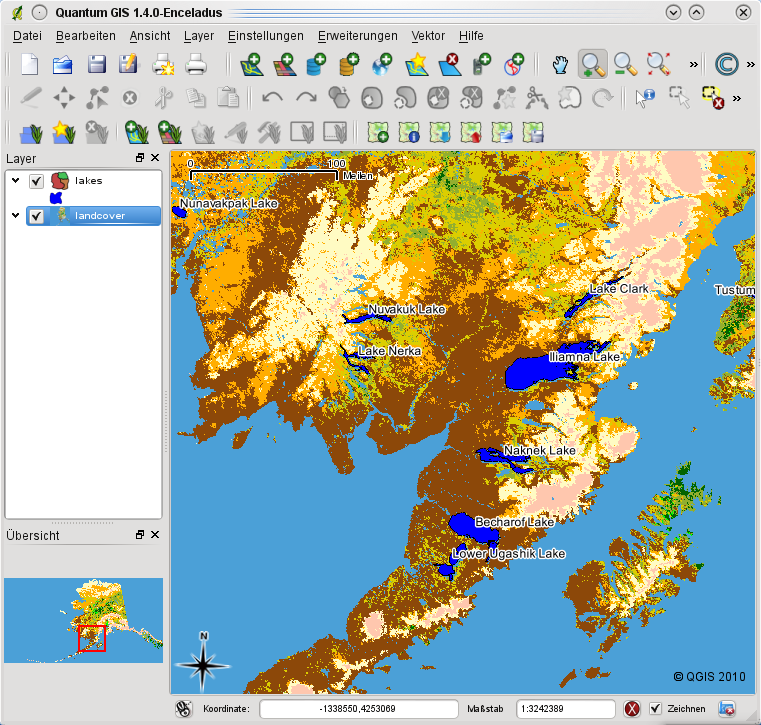
\includegraphics[clip=true, width=14cm]{simple_session} %\end{center}  

%\end{figure} %
%You can see how easy it is to visualize raster and vector layers in  %QGIS. Let's move on to the sections that follow to learn more about the  %available functionality, features and settings and how to use them.

\begin{figure}[ht]
  \begin{center}
    \caption{Une session basique de QGIS \nixcaption}\label{fig:simple_session}\smallskip
    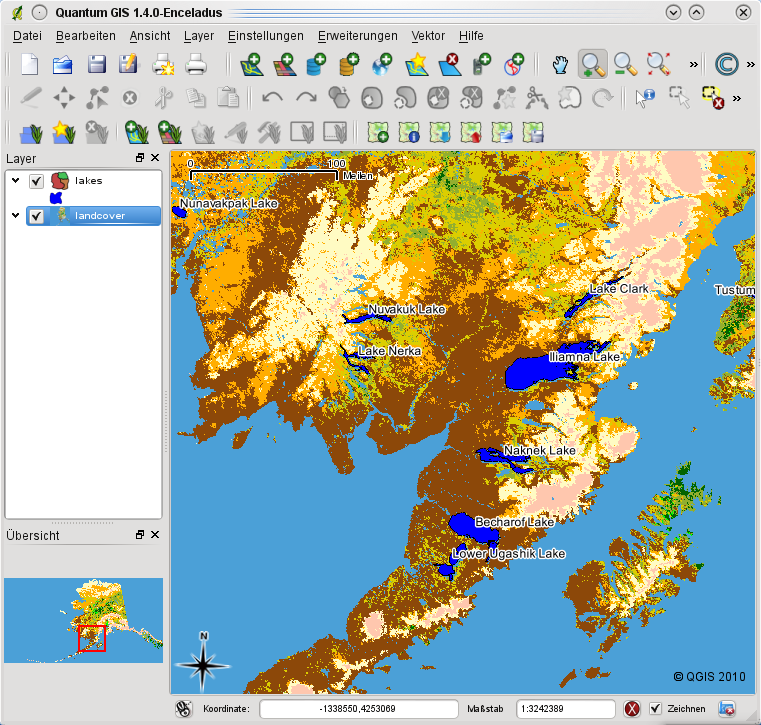
\includegraphics[clip=true, width=14cm]{simple_session}
  \end{center}
\end{figure}

Vous pouvez constater combien il est aisé d'afficher des couches raster ou vecteur dans QGIS. Passons aux sections suivantes pour en apprendre plus sur les autres fonctionnalités et paramètres disponibles et la façon de les utiliser.
